\fancypagestyle{plain}{\fancyhead{}\renewcommand{\headrulewidth}{0pt}}
\chapter{Contesto di sviluppo}
In un contesto di Edge Computing, un ecosistema IoT necessita di tre componenti principali: un dispositivo che raccolga i dati dall'ambiente circostante tramite sensori, un motore di esecuzione in grado di interpretare tali informazioni e un server Cloud (si veda fig. \ref{ecosistema}). All'interno di quest'ultimo sono presenti le descrizioni dei device di interesse e, inoltre, vengono salvati i dati processati dall'engine.

\begin{figure}[H]
	\centering
	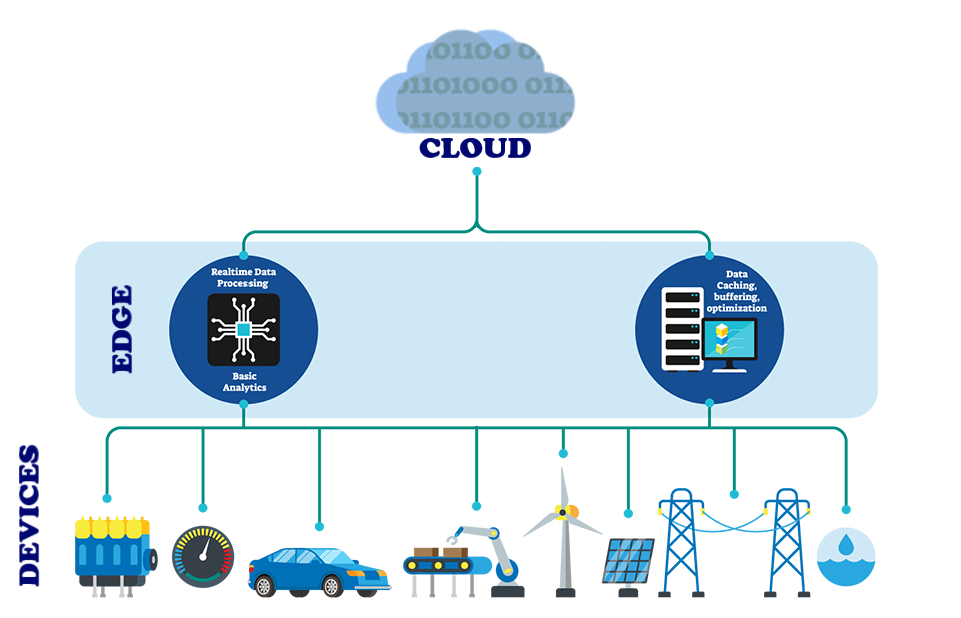
\includegraphics[width=0.8\linewidth]{pics/edgestructure}
	\caption{Ecosistema IoT basato sull'Edge Computing}
	\label{ecosistema}
\end{figure}

\section{Measurify}
Measurify è il server Cloud che è stato impiegato per questo progetto: una piattaforma Cloud-based, astratta e measurement-oriented creata dall'Elios Lab dell'Università degli Studi di Genova per gestire oggetti intelligenti negli ecosistemi IoT. Measurify modella tali oggetti come risorse web esponendole attraverso API che rispettano un'architettura REST (REpresentational State Transfer). In questo modo l'accesso remoto a dati e risorse avviene attraverso un'interfaccia HTTP(S), indipendente dalla piattaforma, per supportare lo sviluppo di applicazioni che si servono di tali oggetti. Le risorse delle API associate al dispositivo specifico sul quale il motore è in esecuzione sono configurabili da remoto con un'applicazione client (ad esempio una web application) che le modifica per gestire l'engine.

Per poter accedere a Measurify sono necessari un username ed una password che permettono di ricevere un token di sicurezza. Nel caso in questione si tratta di un JSON Web Token (JWT), che andrà inserito nell'header di tutte le richieste HTTP(S) successive per garantirne l'autorizzazione.

All'interno di Measurify è presente una struttura descrittiva dei dispositivi associati al proprio username  (si veda fig. \ref{cloudAPI}). Questa è composta da diversi campi che definiscono l'oggetto in questione:

\begin{itemize}
	\item \textbf{Thing}: è  l'oggetto generico che è soggetto a misurazioni da parte dei dispositivi (ad esempio una persona, una macchina, una casa, una città, ecc.);
	\item \textbf{Feature}: è la grandezza fisica misurata da un dispositivo (ad esempio il battito cardiaco, la temperatura ambientale, ecc.);
	\item \textbf{Device}: è un'istanza di una Board usata da una o più applicazioni che
	ha una descrizione virtuale sul Cloud API ;
	\item \textbf{Script}: è un file che contiene informazioni su come l'Edge Engine debba manipolare, memorizzare e trasmettere al cloud gli streams di dati provenienti dai sensori o da altri dispositivi. Può essere una funzione molto complessa per gli engine più potenti oppure un semplice insieme di parametri (ad esempio la velocità di acquisizione o il numero di dati da inviare assieme) per quelli di fascia inferiore;
	\item \textbf{Measurement}: è il valore di una grandezza fisica misurato dal sensore
	di un dispositivo per uno specifico oggetto;
\end{itemize}

\begin{figure}[H]
	\centering
	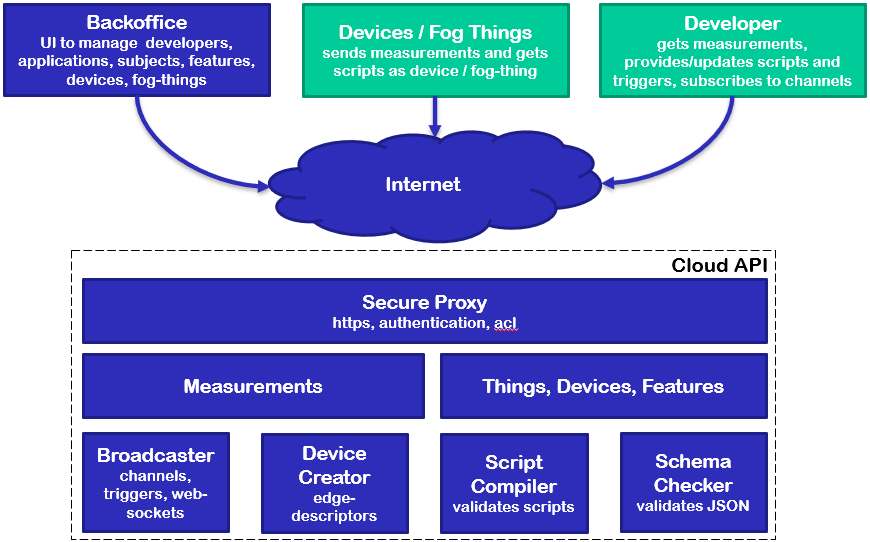
\includegraphics[width=\linewidth]{pics/cloudAPI}
	\caption{Architettura del server Cloud Measurify}
	\label{cloudAPI}
\end{figure}

\section{Edge Engine}
L'Edge Engine è composto da una serie di funzioni unite in un motore di esecuzione che viene eseguito su un host perimetrale. Il progetto è nato inizialmente con lo scopo di essere eseguito su piattaforme di fascia bassa. Di conseguenza, la prima versione ne prevedeva l’utilizzo solo su scheda di sviluppo ESP32-DevKitC V4 con modulo ESP32-WROVER-B su piattaforma Arduino, mantenendo però la possibilità di un futuro adattamento del codice a più dispositivi, come sarà mostrato nel capitolo successivo.

Il funzionamento dell'engine si può riassumere in macro-processi: accesso al Cloud, richiesta della propria descrizione virtuale, richiesta degli scripts da eseguire, lettura dati dai sensori, elaborazione locale dei dati, memorizzazione dei dati e invio degli stessi al Cloud.

L’engine, oltre a username e password necessari per l’accesso al Cloud, deve essere dotato di un identificativo univoco chiamato \textit{id}, inserito all'interno del codice, che gli permetta di identificare ed accedere alla propria rappresentazione virtuale e di specificare la provenienza di tutte le informazioni che andrà a comunicare.

In seguito all'autenticazione, l'engine deve richiedere la propria rappresentazione virtuale, che ne descrive l'identità, i parametri di configurazione e le funzionalità fornendo dunque gli identificativi degli scripts da eseguire. Sul Cloud, per ognuno di questi, deve essere stata in precedenza creata una risorsa di tipo \textit{script} che potrà essere ottenuta dall’engine tramite una GET request. Gli scripts e la descrizione virtuale sono tutti e soli gli elementi di configurazione aggiornabili da remoto. Una volta ottenuti può iniziare la fase operativa.

L’elaborazione locale dei dati raccolti avviene quindi attraverso gli scripts, una composizione di un set predefinito di operazioni semplici, la cui implementazione viene precaricata nell'engine. Queste possono essere applicate agli streams di dati nell'ordine desiderato per formare anche scripts complessi che producono in uscita nuovi streams. L'upload di questi dati sul Cloud può avvenire in due possibili modi: in modo continuo, ovvero il dato viene inviato non appena viene letto e/o processato oppure a lotti, ovvero si può specificare il numero di misure da raggiungere perché queste vengano inviate in blocco dopo essere state memorizzate una ad una.

L'invio dei dati avviene attraverso una POST request sulla rotta delle API dedicata, fornendo nel body della chiamata oltre al dato anche alcune informazioni di tracciabilità, come l'identificativo del dispositivo e dello script che lo ha generato.

Durante l’esecuzione potrebbero verificarsi dei malfunzionamenti che, in questi casi, dovranno essere comunicati dettagliatamente al Cloud, in modo da rendere noto se e quando questi si siano verificati. Così facenso si da anche la possibilità di prendere le dovute contromisure per correggere alcuni errori o semplicemente interpretare correttamente alcune situazioni inaspettate come l'assenza prolungata di comunicazioni verso il server da parte del dispositivo, che potrebbe essere dovuta a molteplici problematiche (connessione, autenticazione fallita, server temporaneamente offline, ecc.).

In figura \ref{edgecloud} è possibile vedere una struttura schematica dell'architettura del sistema Edge Engine - Measurify.

\begin{figure}[H]
	\centering
	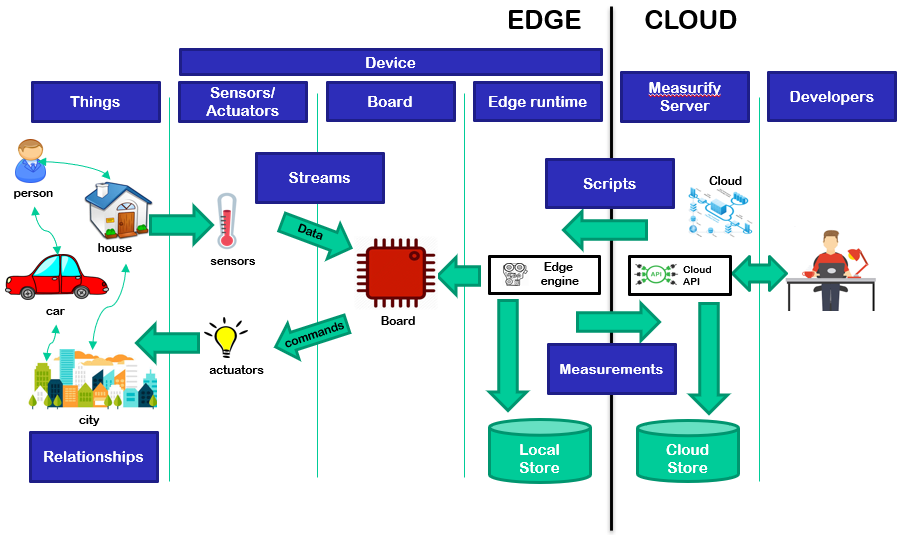
\includegraphics[width=\linewidth]{pics/edgearch}
	\caption{Architettura Edge Engine - Measurify}
	\label{edgecloud}
\end{figure}

\section{Evoluzione del progetto}
A partire dal progetto Edge Engine per Arduino, l’intento è quello di realizzare un prodotto multipiattaforma per dispositivi di tipo PC (Windows/ Linux/ MacOS).

La prima versione di Edge Engine nasce per essere utilizzata esclusivamente su dispositivi Arduino, pertanto, nonostante la maggior parte delle classi sia indipendente dalla piattaforma, ne restano due, \texttt{APIRest} e \texttt{Connection}, specifiche per Arduino. La prima si occupa di gestire le richieste HTTP da e verso il Cloud, mentre la seconda di gestire il modulo WiFi. Entrambe, dal momento che i task che eseguono necessitano di librerie esterne specifiche, sono giocoforza legate alla piattaforma sulla quale vengono eseguite (si veda fig. \ref{arduinodep}). Pertanto, il primo passo per rendere il codice multipiattaforma sarà creare ulteriori classi wrapper \texttt{APIRest\_windows} e \texttt{Connection\_windows}, affinché si generalizzi sempre di più questo aspetto dell'Edge Engine.

\begin{figure}[H]
	\centering
	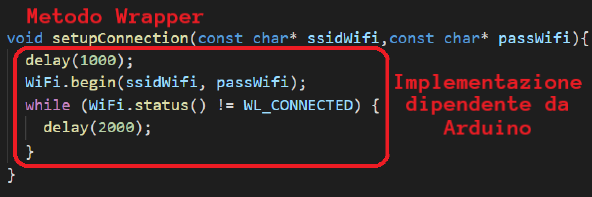
\includegraphics[width=\linewidth]{pics/arduinodependent}
	\caption{Esempio di codice dipendente dalla piattaforma nella classe \texttt{Connection}}
	\label{arduinodep}
\end{figure}

Inoltre, tutte le funzioni specifiche di Arduino utilizzate nel progetto dovranno essere sostituite da funzioni equivalenti per permettere un utilizzo del sistema su dispositivi di tipo PC (ad esempio la funzione \texttt{Serial.print} dovrà essere sostituita da \texttt{cout}).

Nel prossimo capitolo verrà discusso il porting di Edge Engine per dispositivi PC, mantenendo però anche la possibilità di esecuzione su piattaforme Arduino.
